%!TEX root = sm-journal.tex

This section focuses on algorithms that compute strategies for simultaneous move games.
The baseline algorithm for solving simultaneous move games exactly is backward induction~(BI)~(Subsection~\ref{sec:algs:bi}).
%Therefore, we start our description of the algorithms focusing on algorithms based on the backward induction, then we introduce algorithms based on no-regret learning and Monte Carlo sampling.
Afterwards we present a modification that exploits quick calculation of upper and lower bounds in a simultaneous move game~(Subsection~\ref{sec:algs:biab}).
Then, we further improve the algorithm by speeding up the calculation of NE in matrix games, exploiting the iterative framework known as the double-oracle algorithm~(Subsection~\ref{sec:algs:doab}).
In Subsection~\ref{sec:algs:smmcts} we describe Monte Carlo Tree Search for simultaneous move games.
Finally, we present counterfactual regret minimization and its sampling variant outcome sampling in Subsection~\ref{sec:algs:cfros}.


\subsection{Backward Induction}\label{sec:algs:bi}

The standard backward induction algorithm, first described for simultaneous move games in~\cite{Ross71Goofspiel}, is based on the depth-first search that at each state of the game evaluates all successors, creates a matrix game for the current state, solves the matrix game, and propagates back the value of the matrix game. The pseudocode of the algorithm is depicted in Algorithm~\ref{alg:backwardinduction}. If the succeeding node $\cT(s,r,c)$ is a chance node, the algorithm directly evaluates all successors of this chance node computing an expected utility: the value of each subgame rooted in node $s'$ computed by recursive call is weighted by the probability of the stochastic transition $\cP_\star(s,r,c,s')$~(line~\ref{alg:bi:recursive}).

\begin{algorithm2e}[t]
\small
\SetKwInOut{Input}{input}\SetKwInOut{Output}{output}
\Input{$s$ -- current matrix game; $i$ -- searching player}
\If{$s \in \cZ$} {\Return $u_i(s)$} \label{alg:bi:stop1}
\For{$r \in \cA_1(s)$}{
	\For{$c \in \cA_2(s)$} {
	$A_{rc} \leftarrow \sum_{s' \in \cS \;:\; \cP_\star(s,r,c,s') > 0} \cP_\star(s,r,c,s')\cdot \textrm{BI}(s',i)$\label{alg:bi:recursive}\;
	}
}
$\left\langle v_s, \sigma_i(s) \right\rangle \leftarrow$ solve matrix game $A$\;  \label{alg:bi:solve}
\Return $v_s$ \label{alg:bi:stop2}
\caption{Backward Induction algorithm (BI).}\label{alg:backwardinduction}
\end{algorithm2e}

Once the algorithm computes the value of each possible subgame following the current state $s$, the matrix game $A$ is well defined and the algorithm
solves the matrix game $A$ by presenting it as a standard linear program (LP) for solving normal-form games\footnote{\reviewchange{By solving a game we mean computing both the optimal value and the strategy that achieves it.}}:
\begin{eqnarray}
\max & v_s & \\
\textrm{s.t.} & \sum_{a_i \in \cA_{i}}A_{a_i,a_{-i}} \cdot \sigma_i(s,a_i) \geq v_s & \forall a_{-i} \in \cA_{-i}(s)\\
& \sum_{a_{i} \in \cA_{i}} \sigma_i(s,a_{i}) = 1 \\
& \sigma_i(s,a_{i}) \geq 0 & \forall a_{i} \in \cA_{i}(s)
\end{eqnarray}
Using the linear programming, the algorithm computes both the value $v_s$ of the matrix game $A$, as well as strategy to play in this matrix game (variables $\sigma_i(s,a)$).
Value $v_s$ is then propagated to the predecessor~(line~\ref{alg:bi:stop2}) and the optimal strategy $\sigma_i(s,a)$ is stored for this state.
If the algorithm evaluates a terminal state, it directly returns the utility value of the state~(line~\ref{alg:bi:stop1}).

Evaluating each successor and solving an LP in each state of the game is the main computational bottleneck of the backward induction algorithm.
The following algorithms try to prune some of the branches of the game tree in order to reduce this bottleneck even for the price of multiple traversals of the game tree.

\subsection{Backward Induction with Serialized Alpha-Beta Bounds}\label{sec:algs:biab}

Backward induction algorithm can be easily enhanced by using bounds on the value of subgames.
These bounds can be calculated very quickly by using a transformation of a simultaneous move game into a perfect information extensive-form game and applying wide range of search improvements developed for this more standard setting.
Consider a matrix game representing a single simultaneous choice of both players.
This matrix can be serialized by discarding the notion of information sets; hence, letting one player to play first, following by the play of the second player.
The crucial difference between a serialized and a simultaneous move matrix game is that the second player to move has an advantage of knowing what action the first player chose.
\reviewchange{
Given this advantage, the value of a serialized game consisting of a single simultaneous move such that player $i$ is second to move is greater or equal than the value of the original simultaneous move game from the perspective of player~$i$.
Furthermore, we can generalize this argument using induction to game trees with multiple simultaneous moves: when solving a serialized game with $(d+1)$ steps, we know that solving each subgame with $d$ steps acheives an upper bound on the value of that subgame from the perspective of player $i$. 
Therefore, entries in matrix $A$ of the root state are upper bounds on the actual values of the subgames.
By serializing and solving this additional step, we can again get value that is only greater or equal than the value of the original simultaneous move game with $(d+1)$ steps~\cite{Bosansky13Using}.
}
\begin{figure}
\centering
%\begin{tabular}{|l|c|c|}
%\hline $\bigcirc \setminus \square$ & $b_1$ & $b_2$ \\
%\hline $a_1$ & $2$ & $0$ \\
%\hline $a_2$ & $3$ & $4$ \\
%\hline
%\end{tabular}
\begin{tabular}{l|c|c|}
 \multicolumn{1}{c}{~} & \multicolumn{1}{c}{$b_1$}  &  \multicolumn{1}{c}{$b_2$}\\\cline{2-3}
$a_1$ &  2  &  0\\\cline{2-3}
$a_2$ &  3  &  4\\\cline{2-3}
\end{tabular}
\\\vspace{0.5cm}
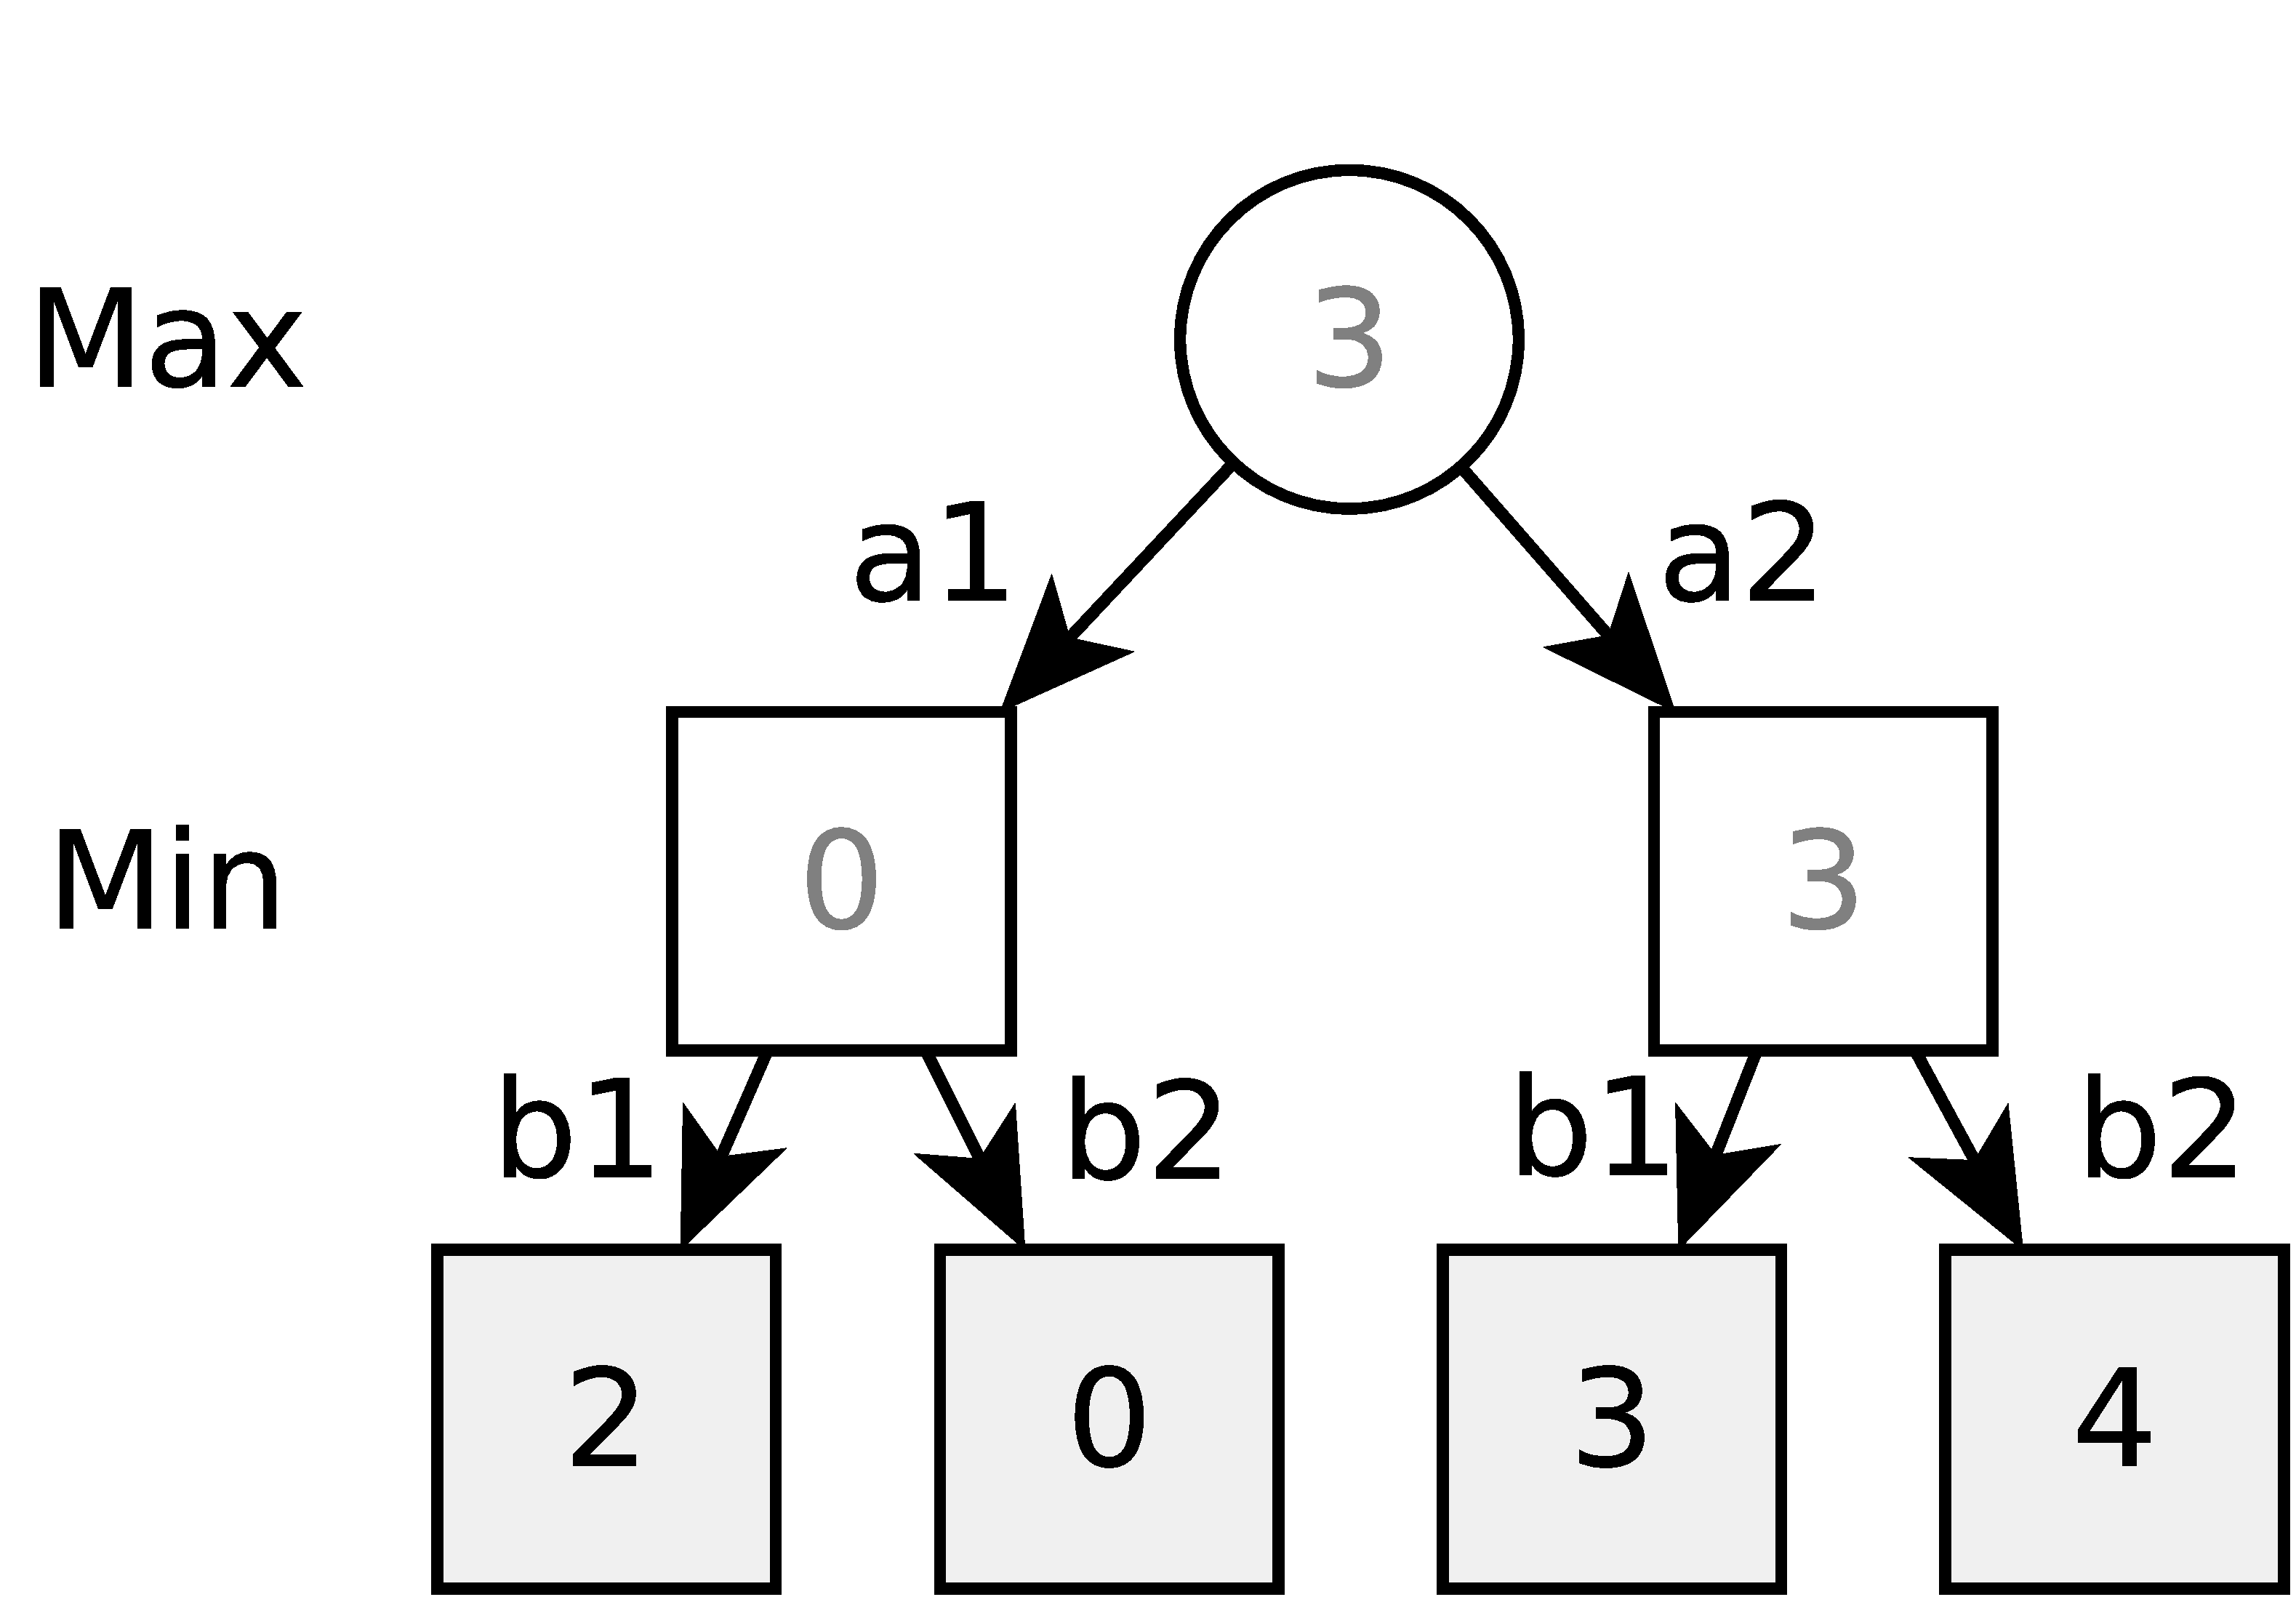
\includegraphics[width=0.35\textwidth]{figures/serialization1.pdf}~~~~~~~
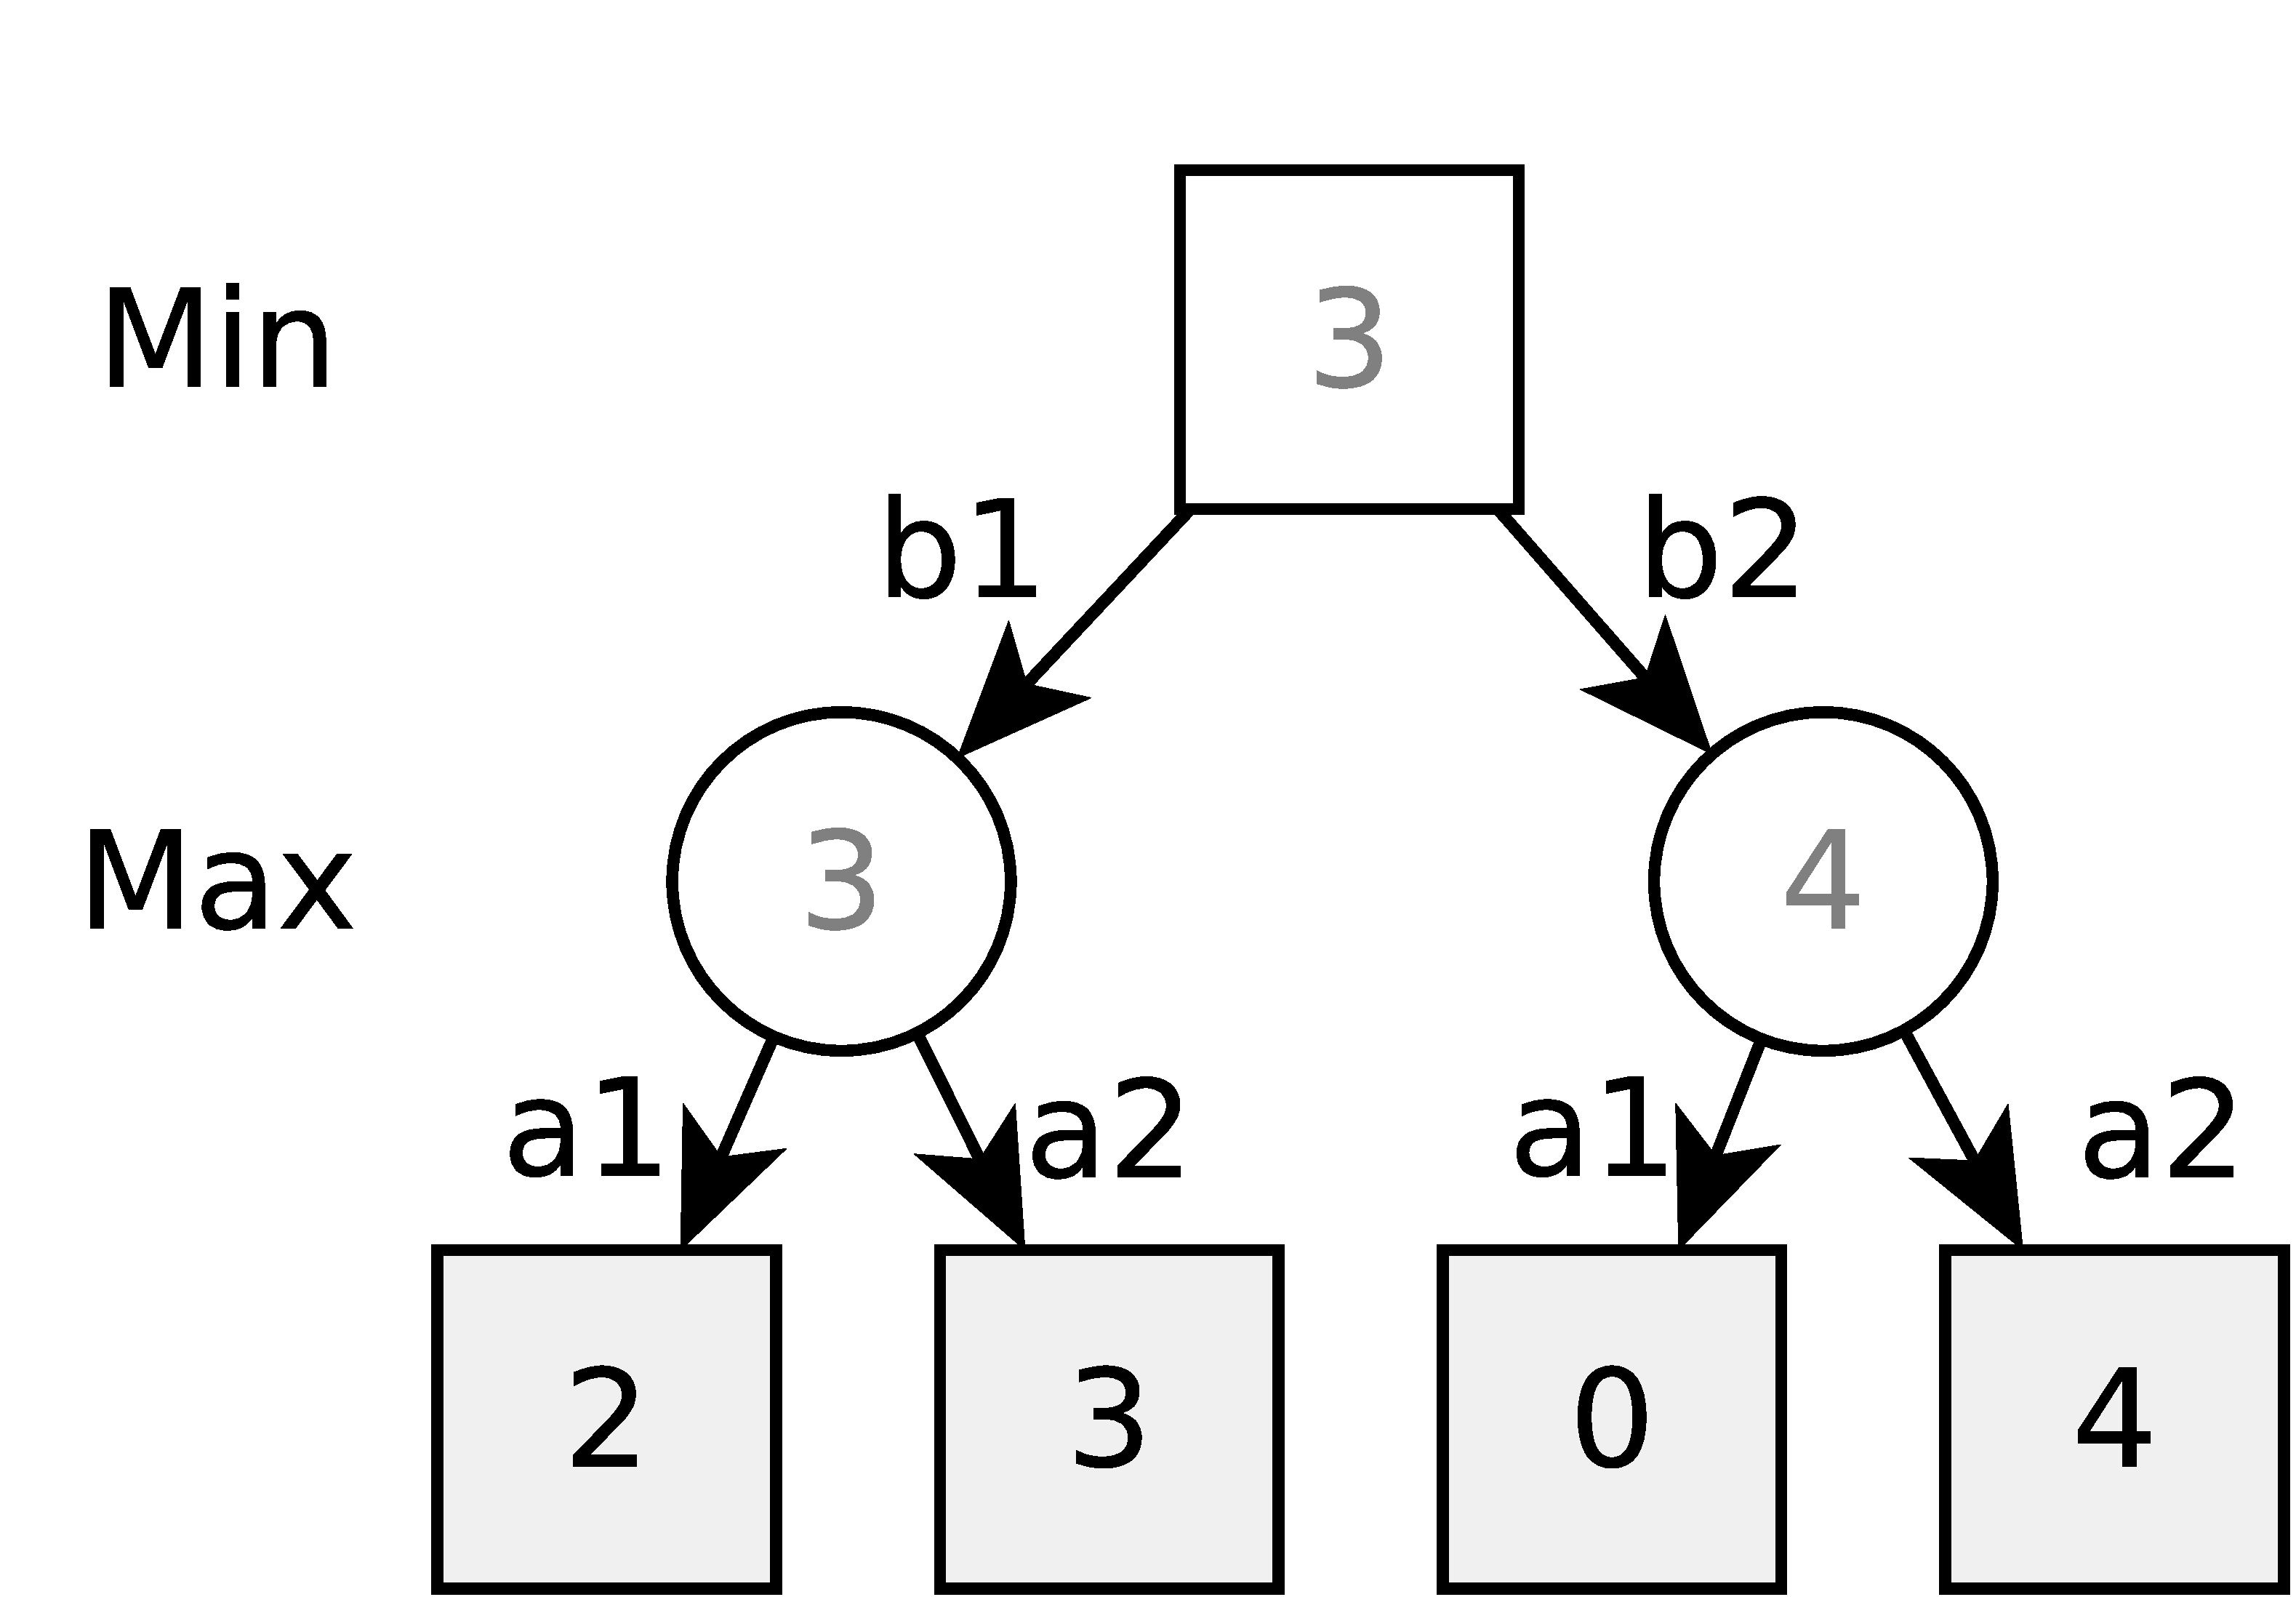
\includegraphics[width=0.35\textwidth]{figures/serialization2.pdf}
\caption{Different serializations of a simultaneous move game. Utility values are in the leafs, the gray values correspond to the value propagation when solving the serialized game.}\label{fig:serialization}
\end{figure}

An example of this serialization is depicted in Figure~\ref{fig:serialization}.
There is a simple matrix game for two players (the circle and the box player; the utility values are depicted for the circle player \ie the box player in the column is minimizing this value) and two ways this game can be transformed into a serialized perfect-information extensive-form game.
If the circle player moves first (the left game tree), then the value of this serialized game is the lower bound of the value of the game. If this player moves second (the right game tree), then the value of this serialized game is the upper bound of the value of the game.
Since the serialized games are zero-sum perfect-information games in the extensive form, they can be solved quite quickly by using a classic AI
algorithm such as alpha-beta or negascout~\cite{Negascout}.
If the values of both serialized games are equal, then this value is also equal to the value of the original simultaneous move game.
This situation occurs in our example in Figure~\ref{fig:serialization}, where both serialized games have value equal to~$3$.

By using bounds calculated in this way we can speed-up the backward induction algorithm (denoted $\biab$).
Algorithm~\ref{alg:backwardinduction-ab} depicts the pseudocode.
\reviewchange{
The algorithm first serializes and solve the whole game using the standard alpha-beta algorithm and returns directly the value from the serialized games if the bounds are equal (line~\ref{alg:biab:stop15}).
The second player to move in the serialization is the player in the argument of the method.}
If the bounds are not equal, the algorithm starts evaluating successors of the current state.
First, the algorithm calculates upper and lower bounds using alpha-beta algorithm on serialized variants of the subgame rooted in the successor $s'$ (lines~\ref{alg:biab:ab1}-\ref{alg:biab:ab2}).
As before, the algorithm uses the value directly if the bounds are equal (line~\ref{alg:biab:saving}), or perform a recursive call otherwise~(line~\ref{alg:biab:recursive}).

We distinguish two cases when extracting the equilibrium strategies from the backward induction with alpha-beta search.
In case that a state was fully evaluated by the algorithm (\ie an LP was built and solved for this state), we proceed as before and keep the pair of equilibrium strategies in this state.
However, in the other case, the algorithms prunes certain branches and does not create an LP for all states.
The algorithm then keeps the strategy calculated by the serialized alpha-beta algorithm.
More precisely, for player~$i$ the algorithm keeps the pure strategy computed by alpha-beta($s$, $-i$), where the opponent has an advantage of knowing the moves of player $i$.
Such a strategy provides guarantees for player~$i$ that is not exploitable and due to the cut-off we know that there is no better strategy for player~$i$ with higher expected utility.
%When such a cut-off occurs, one needs to extract the strategy from alpha-beta.
%Since the alpha-beta operates on a serialized version of the game, the actions played by the player with the additional information caused by observing the choice of his opponent cannot be used.
%This player is not forced to play according to the Nash equilibrium of the original non-serialized game, because the serialized game permits him to choose different action for every choice of the first player.
%And so one needs to extract the strategy for player $i$ from alpha-beta where $i$ plays first. The same goes for the strategy of $-i$.

\begin{algorithm2e}[t]
\small
\SetKwInOut{Input}{input}\SetKwInOut{Output}{output}
\Input{$s$ -- current matrix game; $i$ -- searching player}
\If{$s \in \cZ$} {\Return $u_i(s)$} \label{alg:biab:stop1}
\If{$\left(s\;\textrm{is root}\right)~\mathbf{and}~\left(\textrm{alpha-beta}(s,i) = \textrm{alpha-beta}(s,-i)\right)$} {\Return $\textrm{alpha-beta}(s,-i)$} \label{alg:biab:stop15}
\For{$r \in \cA_1(s)$}{
	\For{$c \in \cA_2(s)$} {
		$A_{rc} \leftarrow 0$\;
		\For{$s' \in \cS \;:\; \cP_\star(s,r,c,s') > 0$} {
		$v^i_{s'} \leftarrow \textrm{alpha-beta}(s',i)$\; \label{alg:biab:ab1}
		$v^{-i}_{s'} \leftarrow \textrm{alpha-beta}(s',-i)$\; \label{alg:biab:ab2}
		\If{$v^{-i}_{s'} < v^i_{s'}$} {
			$A_{rc} \leftarrow A_{rc} + \cP_\star(s,r,c,s')\cdot \textrm{BI}\alpha\beta(s',i)$ \label{alg:biab:recursive}\;
			}
		\Else{
			$A_{rc} \leftarrow A_{rc} + \cP_\star(s,r,c,s')\cdot v^i_{s'}$ \label{alg:biab:saving}
			}
		}
	}
}
$\left\langle v_s, \sigma_i \right\rangle \leftarrow$ solve matrix game $A$\;
\Return $v_s$ \label{alg:biab:stop2}
\caption{Backward Induction with Serialized Bounds $(\biab)$.}\label{alg:backwardinduction-ab}
\end{algorithm2e}

\reviewchange{
The performance of $\biab$ depends on the existence of pure NE in the simultaneous move game.
In the best case (\ie there exists a pure NE), the algorithm finds the solution by solving each serialization exactly once starting from the root state.
The worst case appears, when the only NE requires mixed strategies in each state of the game.
In this case, the algorithm not only solves LP in each state similarly to BI, but also repeatedly solves serialized subgames by calling the alpha-beta algorithm.
In practice, however, this is rarely the case.
}

\subsection{Backward Induction with Double Oracle and Serialized Bounds}\label{sec:algs:doab}

Solving a matrix game can be further improved by using iterative double-oracle algorithm~\cite{McMahan03Planning}.
First of all, we describe the main principles of the double-oracle algorithm in matrix games, following by describing the application of the algorithm in simultaneous move game~\cite{Bosansky13Using} (denoted $\doab$).

\subsubsection{Double-oracle Algorithm for Matrix Games}\label{sec:doab}

The goal of the double-oracle algorithm is to find a solution of a matrix game without necessarily constructing the complete linear program that solves this game.
The main idea is to create a restricted game where the players can only choose from a limited set of actions.
Then, the algorithm iteratively expands the restricted game by allowing the players to choose from new actions.
The new actions are added incrementally; each iteration, a best response to an optimal strategy of the opponent in the current restricted game is
allowed to be played in the restricted game.

Figure~\ref{fig:do-scheme} shows a visualization of the main structure of the algorithm, where the following three steps repeat until convergence:
\begin{enumerate}
\item create a restricted matrix game by limiting the set of actions that each player is allowed to play
\item compute a pair of Nash equilibrium strategies in this restricted game using linear programming
\item for each player, compute a pure best response strategy against the equilibrium strategy of the opponent; pure best response can be \emph{any} action from the original unrestricted game
\end{enumerate}
The best response strategies computed in step 3 are added to the restricted game, the game matrix is expanded by adding new rows and columns, and the algorithm follows with the next iteration. The algorithm terminates if neither of the players can improve the outcome of the game by adding a new strategy to the restricted game; hence, both players play best response strategies to the strategy of the opponent. The algorithm maintains the values of the best expected utilities of the best-response strategies for each player throughout the iterations of the algorithm. These values provide bounds on the value of the original game $V$ (from Equation~\ref{eq:ne}), and their sum represents the error of the algorithm that converges to zero.

\begin{figure}[t!]
\centering
\includegraphics[width=0.9\textwidth]{figures/DO-scheme}
\caption{Schematic of the double-oracle algorithm for a normal-form game.}\label{fig:do-scheme}
\end{figure}

\subsubsection{Integrating Double-Oracle with Backward Induction}

The double-oracle algorithm for matrix games can be directly incorporated into the backward induction -- instead of immediately evaluating each of the successors of the current game state and solving the linear program, the algorithm can exploit the double-oracle algorithm. Pseudocode in Algorithm~\ref{alg:doab} details this integration.
%\mlanctot{Shouldn't the recursive call in 14 of Algorithm \ref{alg:doab} be $\doab(...)$ rather than double-oracle written out?}
%bbosansky: done

\reviewchange{
Similarly to $\biab$, the algorithm first verifies, whether the whole game cannot be solved by using the serialized variants of the game (line~\ref{alg:doab:stop15}).
}
If not, then in each state of the game the algorithm initializes the restricted game with an arbitrary action (line~\ref{alg:doab:init})\footnote{\reviewchange{In practice we use the first action of a shuffled ordered set $\cA_i$ for each player $i$. This initialization step can be improved with domain knowledge by adding more actions.}} -- $A'$ represents the restricted matrix game, $\cA'_i$ represents the restricted set of available actions to player~$i$.
Afterwards, the algorithm starts the iterations of the double-oracle algorithm.
First, the algorithm needs to calculate the value for each of the successors of the restricted game, for which the current value is not known (lines~\ref{alg:doab:restr1}-\ref{alg:doab:saving}). This evaluation is same as in the case of backward induction with alpha-beta algorithm.
Once all values for the restricted game $A'$ are known, the algorithm solves the restricted game (line~\ref{alg:doab:NE}) and keeps the optimal strategies $\sigma'$ of the restricted game.
Next, the algorithm calculates best responses for each of the player~(lines~\ref{alg:doab:br1},\ref{alg:doab:br2}) using Algorithm~\ref{alg:br} below, and updates the lower and upper bounds (line~\ref{alg:doab:bounds}). Finally, the algorithm expands the restricted game with best response actions (line~\ref{alg:doab:expand}) until the lower and upper bound are equal. In this case, neither of the best responses improves the current solution from the restricted game; hence, the algorithm has found an equilibrium of the complete unrestricted matrix game corresponding to state~$s$.

\begin{algorithm2e}[t!]
\small
\SetKwInOut{Input}{input}\SetKwInOut{Output}{output}
\Input{$s$ -- current matrix game; $i$ -- searching player; $\alpha_s,\beta_s$ -- bounds for the game value rooted in state $s$}
\If{$s \in \cZ$} {\Return $u_i(s)$} \label{alg:doab:stop1}
%\If{$v_s^{-i} = v_s^i$} {
%	\Return $v_s^{i}$
%}
%
%\textrm{alpha-beta}(s',i)
%\If{$\alpha_s = \beta_s$} {
%  \Return $\beta_s$
%}
\If{$\left(s\;\textrm{is root}\right)~\mathbf{and}~\left(\textrm{alpha-beta}(s,i) = \textrm{alpha-beta}(s,-i)\right)$} {\Return $\textrm{alpha-beta}(s,-i)$} \label{alg:doab:stop15}
initialize $\cA'_i$, $\cA'_{-i}$ with arbitrary actions from $\cA_i, \cA_{-i}$\; \label{alg:doab:init}
\Repeat{$\alpha_s = \beta_s$}{
	\For{$r \in \cA'_i$, $c \in \cA'_{-i}$}{
		\If{$A'_{rc}$ is not initialized}{\label{alg:doab:restr1}
			 $A'_{rc} \leftarrow 0$\;
			\For{$s' \in \cS \;:\; \cP_\star(s,r,c,s') > 0$} {
			$v^i_{s'} \leftarrow \textrm{alpha-beta}(s',i)$\;
			$v^{-i}_{s'} \leftarrow \textrm{alpha-beta}(s',-i)$\;
			\If{$v^{-i}_{s'} < v^i_{s'}$} {
				$A'_{rc} \leftarrow A'_{rc} + \cP_\star(s,r,c,s')\cdot \doab(s',i,v^{-i}_{s'},v^i_{s'})$\label{alg:doab:recursive}\;
				}
			\Else{
				$A'_{rc} \leftarrow A'_{rc} + \cP_\star(s,r,c,s')\cdot v^i_{s'}$ \label{alg:doab:saving}
				}
			}
		}
	}
	$\left\langle v_s, \sigma' \right\rangle \leftarrow $ solve matrix game $A'$\; \label{alg:doab:NE}
	$\left\langle v^{BR}_i, a^{BR}_{i} \right\rangle \leftarrow $ BR$(s, i, \sigma'_{-i}, \beta_s)$\;\label{alg:doab:br1}
	$\left\langle v^{BR}_{-i}, a^{BR}_{-i} \right\rangle \leftarrow $ BR$(s, -i, \sigma'_{i}, -\alpha_s)$\; \label{alg:doab:br2}
	$\alpha_s \leftarrow \max(\alpha_s, -v^{BR}_{-i})$,
	$\beta_s \leftarrow \min(\beta_s, v^{BR}_{i})$\; \label{alg:doab:bounds}
	$\cA'_i \leftarrow \cA'_i \cup \lbrace a^{BR}_i \rbrace$,
	$\cA'_{-i} \leftarrow \cA'_{-i} \cup \lbrace a^{BR}_{-i} \rbrace$ \label{alg:doab:expand}
}
\Return $v_s$ \label{alg:doab:stop2}
\caption{Double Oracle with Serialized Bounds ($\doab$).} \label{alg:doab}
\end{algorithm2e}


\begin{algorithm2e}[t]
\small
\SetKwInOut{Input}{input}\SetKwInOut{Output}{output}
\Input{$s$ -- current matrix game; $i$ -- best-response player; $\sigma'_{-i}$ -- strategy of the opponent; $\lambda$ -- bound for the best-response value }
$v^{BR}_i \leftarrow \lambda$ \;
$a_i^{BR} \leftarrow \textbf{null}$ \;
\For{$a_i \in \cA_i $\label{alg:br:start}} {%\setminus \cA'_i
	$v_{a_i} \leftarrow 0$\;
	\For{$a_{-i} \in \cA'_{-i} \;:\; \sigma'_{-i}(a_{-i}) > 0$} {\label{alg:br:opp}
    $v_{a_i,a_{-i}} \leftarrow 0$\;
		$\lambda_{a_i} \leftarrow \frac{v_i^{BR} - \sum_{a'_{-i} \in \cA'_{-i} \setminus \lbrace a_{-i} \rbrace} \sigma'_{-i}(a'_{-i}) \cdot v^i_{\cT(s,a_i,a'_{-i})}}{\sigma'_{-i}(a_{-i})}$\; \label{alg:br:bound}
		\If{	$\lambda_{a_i} > v^i_{\cT(s,a_i,a_{-i})}$}{
		continue from line~\ref{alg:br:start} with next $a_i$ \label{alg:br:next}
		}
		\Else{
		\For{$s' \in \cS \;:\; \cP_\star(s,a_i,a_{-i},s') > 0$} {
%			$v^i_{s'} \leftarrow \textrm{alpha-beta}(s',i)$\; \label{alg:br:ab1}
%			$v^{-i}_{s'} \leftarrow \textrm{alpha-beta}(s',-i)$\; \label{alg:br:ab2}
			\If{$v^{-i}_{s'} < v^i_{s'}$} {
				$v_{a_i,a_{-i}} \leftarrow v_{a_i,a_{-i}} + \cP_\star(s,a_i,a_{-i},s')\cdot$ $\doab(s',i,v^{-i}_{s'},v^i_{s'})$\label{alg:br:recursive}\;
				}
			\Else{
				$v_{a_i,a_{-i}} \leftarrow v_{a_i,a_{-i}} + \cP_\star(s,a_i,a_{-i},s')\cdot v^i_{s'}$ \label{alg:br:saving}
				}
			}
			$v_{a_i} \leftarrow v_{a_i} + \sigma'_{-i}(a_{-i})\cdot v_{a_i,a_{-i}}$\;
		}
	}
	\If{$v_{a_i} > v_i^{BR}$}{\label{alg:br:max}
		$v_i^{BR} \leftarrow v_{a_i}$\;
		$a_i^{BR} \leftarrow a_i$\label{alg:br:save}
	}
}
\Return $\langle v_i^{BR}, a_i^{BR} \rangle$
\caption{Best Response with Serialized Bounds (BR)}\label{alg:br}
\end{algorithm2e}

Now we describe the algorithm for calculating the best responses.
The pseudocode of the algorithm is depicted in Algorithm~\ref{alg:br}.
%\mlanctot{Shouldn't the recursive call in 12 of Algorithm \ref{alg:br} be something line BR(...) rather the double-oracle(...)? Also, the function name should be put into the caption as with the other ones.}
%bbosansky: not really, this is actually solving a subgame; hence, DOab is called on the subgame
The goal of the algorithm is to find the best action from the original unrestricted game against current strategy of the opponent $\sigma'_{-i}$.
Throughout the algorithm we use, as before, $v^i_{s'}$ to denote the upper bound of the value of the subgame rooted in state $s'$ calculated using alpha-beta$(s',i)$. These values are calculated on demand, \ie they are calculated once needed and cached until the game for state $s$ is solved.
Moreover, once the algorithm calculates the exact value of a particular subgame, both upper and lower bounds are updated to be equal to actual value of the game.

The algorithm iteratively examines all actions of player $i$ from the unrestricted game (line~\ref{alg:br:start}).
Every action $a_i$ is evaluated against the actions of the opponent that are used in the optimal strategy from the restricted game (line~\ref{alg:br:opp}).
Before evaluating the successors, the algorithm determines, whether current action $a_i$ of the searching player $i$ can still be the best response action against the strategy of the opponent $\sigma'_{-i}$.
\reviewchange{In order to determine this, the algorithm computes value $\lambda_{a_i}$ that represents the lower bound on the expected utility this action must gain against the current action of the opponent $a_{-i}$ in order for action $a_i$ to be the best response.
$\lambda_{a_i}$ is calculated (line~\ref{alg:br:bound}) by subtracting upper bound of the expected value against all other actions of the opponent ($v^i_{\cT(s,a_i,a'_{-i})}$) from the current best response value ($v_i^{BR}$) and normalizing with the probability that the action $a_{-i}$ is played by the opponent ($\sigma'_{-i}(a_{-i})$).
This calculation corresponds to situation when player $i$ achieves the best possible utility by playing action $a_i$ against all other actions from the strategy of the opponent and it needs to achieve at least $\lambda_{a_i}$ against $a_{-i}$ so that expected value for playing $a_i$ is at least $v_i^{BR}$.}
%The value $\lambda_{a_i}$ represents the lowest possible expected utility this action must gain against the current action of the opponent $a_{-i}$.
If value $\lambda_{a_i}$ is strictly higher than the upper bound on the value of the subgame rooted in the successor (\ie $v^i_{\cT(s,a_i,a_{-i})}$) then the algorithm knows that the action $a_i$ can never be the best response action, and can proceed with the next action (line~\ref{alg:br:next}).
\reviewchange{Note that $\lambda_{a_i}$ is recalculated for each action of the opponent since the upper bound values can become tighter when the exact values are computed for successor nodes $s'$ (line~\ref{alg:br:recursive}).}
%

If the currently evaluated action $a_i$ can still be the best response, the value of the successor is determined (first by comparing the bounds). Once the expected outcome against all actions of the opponent is known, the expected value of action $a_i$ is compared against the current best-response value (line~\ref{alg:br:max}) and saved, if the expected utility is higher~(line~\ref{alg:br:save}). The best response actions are allowed in the next iteration of the double-oracle algorithm and the algorithm progresses further as described.

When extracting strategies from the double-oracle algorithm with serialized alpha-beta, we proceed exactly as in the case of $\biab$: either a double-oracle is initialized and solved for certain matrix game and we keep equilibrium strategies from the final restricted game, or the strategy is extracted from the serialized alpha-beta algorithms as before.

\reviewchange{
Similarly to $\biab$, the performance of $\doab$ also depends on the existence of pure NE in the simultaneous move game.
The best case is identical to $\biab$ and the algorithm finds the solution by solving each serialization exactly once starting from the root state.
In the worst case, none of the serialized games yield useful bounds and the algorithm needs to call the double-oracle algorithm in every state.
Moreover, the worst case for the double-oracle algorithm is such that all actions in this state must be added and only a single action is added in each iteration causing the largest number of iterations repeatedly resolving the linear program.
Again in practice, however, this is rarely the case.
Moreover, the computational overhead from repeatedly solving a LP is relatively small in practice.
This is due to the size of each LP that is determined by the number of actions in each state (number of constraints and variables is bounded by the number of actions in each state).
Therefore, the size of each LP is small compared to the number of states $\doab$ can prune out, especially if the pruning occurs close to the root of the game tree.
}

\subsection{Simultaneous Move Monte Carlo Tree Search (SM-MCTS)} \label{sec:algs:smmcts}

%\bbosansky{It seems to me that the two parts (BI / sampling) are quite uneven in terms of details and readability. The first part is quite verbose with examples, while MCTS and OOS are quite condensed and more difficult to follow. It would be good to rewrite add some more text description and intuition into MCTS/OOS (it is encouraged in the AIJ submission info to be less heavy and provide intuition).}
%\mlanctot{Agree. I will do this.}

In the following subsections we move to approximative algorithms.
Monte Carlo Tree Search (MCTS) is a simulation-based state space search algorithm often used
in game trees. The nodes in the tree represent game states. The main idea is to iteratively run
simulations to a terminal state, incrementally growing a tree rooted at the initial state of the game. In
its simplest form, the tree is initially empty and a single leaf is added each iteration. Each iteration
starts by visiting nodes in the tree, selecting which actions to take based on a \emph{selection function} and
information maintained in the node. Consequently, the algorithm transitions to a successor state. When a
node is visited whose immediate children are not all in the tree, the node is expanded by adding a
new leaf to the tree. Then, \emph{a rollout policy} (\eg random action selection) is applied from the new
leaf to a terminal state. The outcome of the simulation is then returned as a reward to the new leaf
and the information stored in the tree is updated.

\begin{figure}[t]
\centering
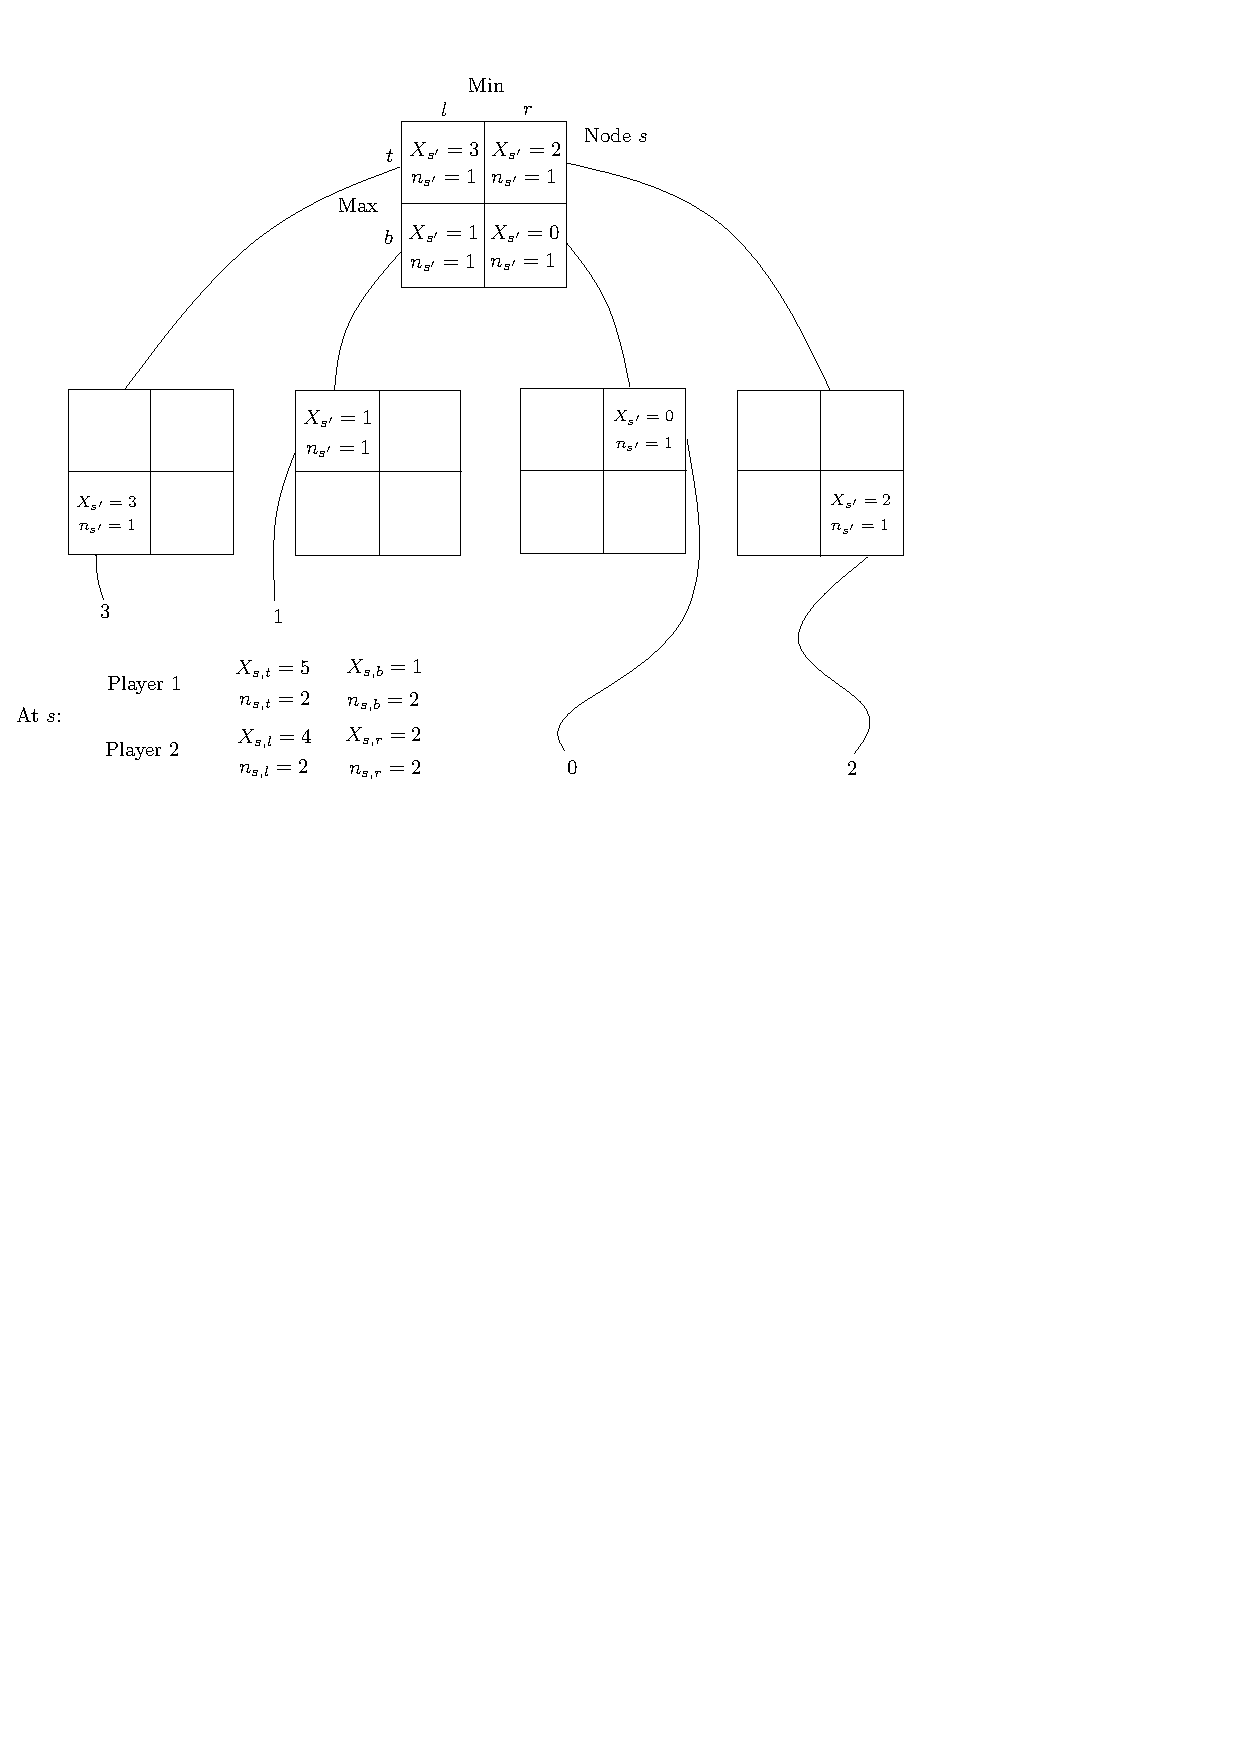
\includegraphics[scale=0.7]{figures/smmcts-example}
\caption{Simultaneous Move MCTS example.
Here, $X_{s'}$ represents the cumulative payoff of all simulations that have passed
through the cell, while $n_{s'}$ represents the number of simulations that have passed through the cell.}
\label{fig:smmcts-example}
\end{figure}

Consider again the game depicted in Figure~\ref{fig:example}. We demonstrate how Monte Carlo Tree Search
could progress in this game using the example shown in Figure~\ref{fig:smmcts-example}. This game has a root state,
two subgames that are simple matrix games and two arbitrarily large subgames. In the root state, player 1 (Max) has two
actions: top ($t$) and bottom ($b$), and player 2 also has two actions: left ($l$) and right ($r$). The tree is initialized
with a single empty state, $s$. On the first iteration, the first child corresponding to $(t,l)$ is added to the tree,
giving a payoff $u_1 = 3$ at the terminal state which is backpropagated to each state visited on the simulation.
Similarly, on the second iteration the second child corresponding to $(b,l)$ is added to the tree, giving a payoff $u_1 = 1$ is
backpropagated up to all of its parents.
After four simulations, every cell in the root state has a value.

\begin{algorithm2e}[t]
\small
\SetKwInOut{Input}{input}\SetKwInOut{Output}{output}
\Input{$s$ -- current state of the game}
\If{$s \in \cZ$} {
	\Return $u_1(s)$\;
}
\If{$s \in \cC$ is a chance node} {
        Sample $s' \sim \Delta_\star(s)$\;
	\Return SM-MCTS($s'$)\;
}
\If{$s$ is in the MCTS tree} {
	$(a_1, a_2) \leftarrow$ \emph{\underline{Select}}$(s)$\;\label{alg:smmcts:select}
	$s' \leftarrow \cT(s,a_1,a_2)$\;
	$v_{s'} \leftarrow $ SM-MCTS($s'$)\;\label{alg:smmcts:reccall}
	\emph{\underline{Update}}$(s,a_1,a_2,v_{s'})$\;\label{alg:smmcts:up}
	\Return $v_{s'}$\;
}
\Else{
	Add $s$ as a new child in the MCTS tree\;
	$v_{s} \leftarrow$ Rollout($s$)\;\label{alg:smmcts:rollout}
	\Return $v_{s}$\; \label{alg:smmcts:return}
}
\caption{Simultaneous Move Monte Carlo Tree Search (SM-MCTS)}\label{alg:smmcts}
\end{algorithm2e}

There are many possible ways to select actions based on the estimates stored in the each cell which lead to different variants.
We therefore first formally describe a generic template of MCTS algorithms for simultaneous move games (SM-MCTS) and then explain specific algorithms derived from this template.
Algorithm~\ref{alg:smmcts} describes a single iteration of SM-MCTS.
The ``MCTS tree'' is an explicit tree data structure that stores the nodes of the search tree maintained in memory,
\eg the five-node tree shown in Figure~\ref{fig:smmcts-example}.
% mlanctot: actually I hardly used it so I just wrote it out explicitly, one less symbol to remember
%\bbosansky{I'd use $\cS'$ or something based on $\cS$ instead of $T$.}
Every node $s$ in the tree maintains algorithm-specific statistics about the iterations that previously used this node.
The template can be instantiated by specific implementations of the updates of the statistics on line~\ref{alg:smmcts:up} and the selection based on these statistics on line \ref{alg:smmcts:select}.
In the terminal states, the algorithm returns the value of the state for the first player (line 2).
In the chance nodes, the algorithm selects one of the possible next stated based on the chance distribution (line 4).
If the current state has a node in the current MCTS tree, the statistics in the node are used to select an action for each player (line~\ref{alg:smmcts:select}).
These actions are executed (line 8) and the algorithm is called recursively on the resulting state (line 9).
The result of this call is used to update the statistics maintained for state $s$ (line~\ref{alg:smmcts:up}).
If the current state is not stored in tree, it is added to the tree (line 13) and its value is estimated using the rollout policy (line 14).

Different algorithms can be the bases for the selection functions (\eg UCB~\cite{UCB}, Exp3~\cite{Auer2003Exp3}, and regret-matching~\cite{Hart00}).
We now present the variants of SM-MCTS that were consistently the most successful in the previous works,
though more variants can be found in~\cite{Perick12Comparison,Lanctot13Tron,Tak14smmcts}.

\subsubsection{Decoupled Upper-confidence Bound applied to Trees}\label{sec:duct}

The most common selection function for SM-MCTS is the decoupled Upper-Confidence Bound applied to Trees (UCT).
For selection and updates, it executes the well-known UCT \cite{UCT} algorithm independently for each of the players in each nodes.
The statistics stored in search nodes are independently computed for each action of each player. For player $i\in \cN$ and
action $a_i \in \cA_i(s)$ the reward sums $X_{a_i}$ and the number of times the action was used $n_{a_i}$ are maintained.
When a joint action needs to be selected by the \emph{\underline{Select}} function, an action that maximizes the UCB value over
their reward estimates is selected for each player independently (therefore it is called decoupled):
\begin{equation}
a_i = \argmax_{a_i \in \cA_i(s)}{ \left\{ \bar{X}_{a_i} + C_i \sqrt{\frac{\log n_s}{n_{a_i}}} \right\} },
  \mbox{ where } \bar{X}_{a_i} = \frac{X_{a_i}}{n_{a_i}} \mbox{ and } n_s=\sum_{b_i \in \cA_i(s)} n_{b_i}.\label{eq:uct}
\end{equation}
\noindent The \emph{\underline{Update}} function increases the visit count and rewards for each player $i$ and its selected action $a_i$ using $X_{a_i} \leftarrow X_{a_i} + u_i$
and $n_{a_i} \leftarrow n_{a_i} + 1$.

Consider again the example shown in Figure~\ref{fig:smmcts-example}. Decoupled UCT now groups together all the payoffs obtained
for an action. Therefore, at the root Max has $\bar{X}_t = 5/2 = 2.5, \bar{X}_b = 1/2 = 0.5$ and the exploration term for both is
$C_i \sqrt{(\log 4) / 2}$, and so top is selected. For Min, $\bar{X}_l = 3/2 = 1.5 = \bar{X}_r$, so both actions have the same value.
\reviewchange{So, in this situation Min must use a tie-breaking rule to decide which action to take.
As we show in Subsection~\ref{sec:exp:brps}, the specific tie-breaking rule used here could lead to a significant effect on the quality
of the strategy UCT produces.}

After all the simulations are done, there are two options how to determine the resulting action to play.
The more standard option is to choose for each state the action $a_i$ that maximizes $n_{a_i}$ for each player $i$.
This is suitable mainly for games, in which using mixed strategy is not necessary.
Alternatively, the action to play in each state can be determined based on the mixed strategy obtained by normalizing the visit counts of each action
\begin{equation}
\sigma_i(a_i) = \frac{n_{a_i}}{\sum_{b_i\in \cA_i(s)} n_{b_i}}.
\label{eq:ductmix}
\end{equation}
Using the first method certainly makes the algorithm not converge to a Nash equilibirum, because the game may require a mixed strategy.
Therefore, unless stated otherwise, we only use the mixed form in Equation~\ref{eq:ductmix}.% from now on and refer to this algorithm simply as UCT.

Note, however, it was shown that this latter variant also might not converge to a Nash equilibrium (a well known counter-example in Rock, Paper, Scissors with biased payoffs~\cite{Shafiei09}).
However, one of the issues when using UCT in game trees is an underspecified behavior in case there are multiple actions with identical value in the maximization described in the UCT formula in Equation~\ref{eq:uct}.
%Note that UCT does not define what happens which action is selected if multiple actions have identical value in the maximization.
This may have a significant impact on the performance of the UCT in simultaneous move games.
Consider the matrix game at the right of Figure~\ref{fig:egMatrixGames}.
This game has only one NE, such that both players play the first action. However, UCT selecting the first or the last action among the options with the same value will always get only the rewards 0 and the bias term will cause the players to round-robin over the diagonal indefinitely. This is clearly not optimal, as each player can than improve by playing first action with probability 1. However, if we choose the action to play randomly among the tied actions (where ``tied'' could be defined as being within a small tolerance gap), UCT will quickly converge to the optimal solution in this game.
We will experimentally analyze the impact of this randomization on the example used in~\cite{Shafiei09} and show that if a randomized variant of UCT is used, the algorithm still does not converge to a NE but does converges to a strategy that is much closer to a NE than without randomization (see Subsection~\ref{sec:exp:brps}).
Therefore, unless stated otherwise, we use the randomized variant in our implementation.

Even though UCT is not guaranteed to converge to the optimal solution, it is often very successful in practice.
It has been used in and general game playing~\cite{Finnsson12}, in the card game Urban Rivals~\cite{Teytaud11Upper},
and in Tron~\cite{Perick12Comparison}.

% mlanctot: removed, was confusing.
%Note that UCT described in this section is different than UCT run on a game that is transformed to perfect information by serialization of the simultaneous moves, because in the latter case one player has the advantage of knowing what the other player chose at every stage.
%\vlisy{Possibly mention convergence in games with pure strategies.}\bbosansky{I'd remove this last sentence of this para.}

\subsubsection{Exponential-weight algorithm for Exploration and Exploitation}\label{sec:exp3}

Another common choice is to use the Exponential-weight algorithm for Exploration and Exploitation (Exp3)
algorithm \cite{Auer2003Exp3} independently for each of the players.
In Exp3, each player maintains an estimate of the sum of rewards for each action, denoted $\hat{X}_{a_i}$.
The joint action produced by \emph{\underline{Select}} is composed of an action independently selected for each player.
An action is selected by sampling from a probability distribution over actions.
Define $\gamma$ to be the probability of exploring, \ie choosing an action uniformly.
The probability of selecting action $a_i$ is proportional to the exponential of the reward estimates:
\begin{equation}\label{eq:exp3select}
\sigma_i(a_i) = \frac{(1-\gamma) \exp(\eta \hat{X}_{a_i})}{\sum_{b_i \in \cA_i(s)} \exp(\eta \hat{X}_{b_i})} + \frac{\gamma}{|\cA_i(s)|},
  \mbox{ where } \eta = \frac{\gamma}{|\cA_i(s)|}.
\end{equation}

This standard formulation of Exp3 is suitable for deriving its properties, but a straightforward implementation of this formula leads to problems with numerical stability. Both the numerator and denominator of the fraction can quickly become too large. For this reason, other formulations have been suggested, \eg in \cite{Lanctot13Goofspiel} and \cite{Cowling12ISMCTS} that are more numerically stable. We use the following equivalent formulation from \cite{Cowling12ISMCTS}:
\begin{equation} \label{eq:exp3:stable}
\sigma_i(a_i) = \frac{(1-\gamma)}{\sum_{b_i \in A_i(s)}\exp(\eta(\hat{X}_{b_i}-\hat{X}_{a_i}))} + \frac{\gamma}{|\cA_i(s)|}.
\end{equation}

The update after selecting actions $(a_1,a_2)$ and obtaining a simulation result $v_1$ normalizes the result to the unit interval for each player by
\begin{equation}
u_1 \leftarrow \frac{(v_1 - v_{min})}{v_{max} - v_{min}};\;\; u_2 \leftarrow (1-u_1)
\end{equation}
and adds to the corresponding reward sum estimates the reward divided by the probability that the action was played by the player using
\begin{equation}
\hat{X}_{a_i} \leftarrow \hat{X}_{a_i} + \frac{u_i}{\sigma^t_i(a_i)}.
\end{equation}
Dividing the value by the probability of selecting the corresponding action makes $\hat{X}_{a_i}$ estimate the sum of rewards over all
iterations, not only the ones where $a_i$ was selected.

As the final strategy, after all iterations are executed, the algorithm computes the \emph{average strategy} of the Exp3 algorithm over all iterations for each player.
\reviewchange{Let $\sigma^t_i$ be the strategy used at time $t$.} After $T$ iterations in the particular node, it is
\begin{equation}
\bar{\sigma}^T_i(a_i) = \frac{1}{T}\sum_{t=1}^T \sigma^t_i(a_i).
\end{equation}
In our implementation, we maintain the cumulative sum and normalize it to obtain the average strategy after the iterations.

Previous work \cite{Teytaud11Upper} suggests first removing the samples caused by the exploration.
This modification proved to be useful also in our experiments
% and it has been shown not to reduce the performance substantially in the worst case \cite{kovarik}, \mlanctot{@Vilo, please add the missing reference; I don't know which paper you wanted to cite here}
so as the resulting final mixed strategy, we use
\begin{equation}
\bar{\sigma}_i(a_i) \leftarrow \max\left(0, \bar{\sigma}_i(a_i) - \frac{\gamma}{|\cA_i(s)|}\right),
\end{equation}
normalized to sum to one.

\subsubsection{Regret Matching} \label{sec:rm}

This variant applies regret matching \cite{Hart00} to the current estimated matrix game at each stage and was first used in~\cite{Lanctot13Goofspiel}. The statistics stored by this algorithm in each node are the use count of each joint action ($n_{a_1a_2}$), the sum of rewards for each joint action ($X_{a_1a_2}$).\footnote{Note that $n_{a_1a_2}$ and $X_{a_1a_2}$ correspond to $n_{s'}$ and $X_{s'}$ from Figure~\ref{fig:smmcts-example}.}
Furthermore, the algorithm for each player $i$ maintains a cumulative regret $r^i_{a_i}$ for having played $\sigma_i^t$ instead of $a_i \in \cA_i(s)$ on iteration $t$, initially set to 0. The regret values $r^i_{a_i}$ are maintained separately by each player. However, the updates use a value that is a function of the joint action space.

On iteration $t$, function \emph{\underline{Select}} first builds
each player's current strategies from the cumulative regrets. Define $x^+ = \max(x,0)$,
\begin{equation}
\label{eq:rm}
\sigma_i(a_i) = \frac{r^{i+}_{a_i}}{R^+_{sum}} \mbox{ if } R^+_{sum} > 0
\mbox{ oth. } \frac{1}{|\cA_i(s)|}, \mbox{ where } R^+_{sum} = \sum_{b_i \in \cA_i(s)}{r^{i+}_{b_i}}.
\end{equation}
The main idea is to adjust the strategy by assigning higher weight proportionally to actions based on the regret of having not taken them over the long-term.
To ensure exploration, a sampling procedure similar to Equation~\ref{eq:exp3select} is used to select action $a_i$ with probability
$\gamma/|\cA_i(s)| + (1-\gamma) \sigma_i(a_i)$.

\emph{\underline{Update}} adds regret accumulated at the iteration to
the regret tables $r^i$. Suppose joint action $(a_1,a_2)$ is
sampled from the selection policy and utility $u_1$ is returned from the recursive call on line~\ref{alg:smmcts:reccall}.
Label $reward(b_1,b_2) = \frac{X_{b_1b_2}}{n_{b_1b_2}}$ if
$(b_1,b_2) \not= (a_1,a_2)$, or $u_1$ otherwise. The updates to the regret are:
\begin{eqnarray}
\forall b_1 \in \cA_1(s), ~~  r^1_{b_1} \leftarrow r^1_{b_1} + ( reward(b_1, a_2) - u_1 ),\\
\forall b_2 \in \cA_2(s), ~~  r^2_{b_2} \leftarrow r^2_{b_2} - ( reward(a_1, b_2) - u_1).
\end{eqnarray}
%\noindent and average strategy updates for each player, $\bar{\sigma}^i_s[a] \leftarrow \bar{\sigma}^i_s[a] + \sigma^t_i(s,a).$

After all simulations, the strategy to play in state $s$ is defined by the mean strategy used in the corresponding node as in case of Exp3.

\subsection{Counterfactual Regret Minimization and Outcome Sampling} \label{sec:algs:cfros}

Finally, we describe algorithms based on Counterfactual Regret (CFR; a notion of regret at the information set level),
first designed for extensive-form games with imperfect information~\cite{CFR} and first applied to simultaneous move games in~\cite{Lanctot13Goofspiel}.

\reviewchange{Recall from Section~\ref{sec:smg} the set of histories $\cH$. Here we also use $\cZ$ defined previously as the set of terminal states,
to refer to the set of {\it terminal histories} since there is a one-to-one correspondence between them.}
A {\it history} as a sequence of actions taken by all players (including chance) that starts from the beginning of the game.
A history $h'$ is a prefix of another history $h$, denoted $h' \sqsubset h$, if $h$ contains $h'$ as a prefix sequence of actions.
The {\it counterfactual value} of reaching information set $I$ is the expected payoff given that player $i$ played to reach $I$, the opponents played
$\sigma_{-i}$ and both players played $\sigma$ after $I$ was reached:
\begin{equation}
\label{eq:cfv}
v_i(I,\sigma) = \sum_{(h,z) \in \cZ_I} \pi^{\sigma}_{-i}(h) \pi^{\sigma}(h,z) u_i(z),
\end{equation}
where $\cZ_I = \{ (h,z)~|~z \in \cZ, h \in I, h \sqsubset z \}$, \reviewchange{$\pi^{\sigma}_{-i}(h)$ is the product of probabilities to reach $h$ under $\sigma$ excluding player $i$'s (i.e., including nature)\bbosansky{TODO @Marc -- I have added ``(i.e., including nature)'' so just checking. Remove, this note if it is OK.},
and $\pi^\sigma(h,h')$, where $h \sqsubset h'$, is the probability of all actions taken along the path from $h$ to $h'$.}
Suppose, at time $t$, players player with strategy profile $\sigma^t$.
Define $\sigma^t_{I \rightarrow a}$ as identical to $\sigma^t_i$ except at $I$ action $a$ is taken with probability $1$.
Player $i$'s counterfactual regret of not taking $a \in \cA(I)$ at time $t$ is $r_i^t(I,a) = v_i(I, \sigma^t_{I \rightarrow a}) - v_i(I,\sigma^t)$.
The CFR algorithm maintains the cumulative regret $R_i^T(I,a) = \sum_{t=1}^T r_i^t(I,a)$, for every action at every information set.
Then, the distribution at each information set for the next iteration $\sigma^{T+1}(I)$ is obtained individually using
regret-matching~\cite{Hart00}. The distribution is proportional to the positive portion of the individual actions' regret:
\begin{equation*}
\label{eq:rm}
\sigma^{T+1}(I,a) = \left\{
\begin{array}{ll}
R_i^{T,+}(I,a) / R^{T,+}_{i,sum}(I) & \mbox{if } R^{T,+}_{i,sum}(I) > 0 \\
1 / |\cA(I)|                   & \mbox{otherwise,}
\end{array} \right.
\end{equation*}
where $x^+ = \max(0,x)$ for any term $x$, and $R^{T,+}_{i,sum}(I) = \sum_{a' \in A(I)} R_i^{T,+}(I,a')$.
Furthermore, the algorithm maintains for each information set the average   strategy profile
\begin{equation}
%\bar{\sigma}^T(I,a) = \frac{1}{T}\sum_{t=1}^T \sigma^t(I,a).
\bar{\sigma}^T(I,a) = \frac{\sum_{t=1}^T \pi^{\sigma^t}_i(I) \sigma^t(I,a)}{\sum_{t=1}^T \pi^{\sigma^t}_i(I)},
\end{equation}
where $\pi^{\sigma^t}_i(I) = \sum_{h \in I}\pi^{\sigma^t}_i(h)$.
The combination of the counterfactual regret minimizers in individual information sets also minimize the overall
average regret \cite{CFR}, and hence due to the Folk Theorem the average profile is a  $2\epsilon$-equilibrium,
with $\epsilon \rightarrow 0$ as $T \rightarrow \infty$.

Monte Carlo Counterfactual Regret Minimization (MCCFR) applies CFR to sampled portions of the games~\cite{Lanctot09Sampling}.
In the {\it outcome sampling} (OS) variant, a single terminal history $z\in \cZ$ is sampled in each iteration.
The algorithm updates the regret in the information sets visited along $z$ using the
{\it sampled counterfactual value},
\begin{equation}
\tilde{v}_i(I,\sigma) = \left\{
\begin{array}{ll}
\frac{1}{q(z)} \pi^{\sigma}_{-i}(h) \pi^{\sigma}(h,z) u_i(z) & \mbox{if } (h,z) \in \cZ_I\\
0  & \mbox{otherwise,}
\end{array} \right.
\label{eq:scv}
\end{equation}
where $q(z)$ is the probability of sampling $z$.
As long as every $z \in Z$ has non-zero probability of being sampled, $\tilde{v}_i(I,\sigma)$ is an unbiased estimate of $v(I,\sigma)$
due to the importance sampling correction ($1/q(z)$). For this reason, applying CFR updates using these sampled counterfactual regrets
$\tilde{r}_i^t(I,a) = \tilde{v}_i(I,\sigma^t_{I \rightarrow a}) - \tilde{v}_i(I,\sigma^t)$
on the sampled information sets values also eventually converges to the approximate equilibrium of the game with high probability.
The required number of iterations for convergence is much larger, but each iteration is much faster.

%Pseudocode of outcome sampling is presented in the next subsection.

% Will put pseudocode in the Online part..?
%\begin{algorithm2e}[t]
%\small
%\SetKwInOut{Input}{input}\SetKwInOut{Output}{output}
%\Input{game $g$}
%\Return 1
%\caption{Outcome Sampling MCCFR}\label{alg:os}
%\end{algorithm2e}

\subsubsection{Online Outcome Sampling} \label{sec:oos}

We now present Online Outcome Sampling (OOS) for simultaneous move games. Note, importantly, that OOS is different from the general SM-MCTS
algorithms presented in Subsection~\ref{sec:algs:smmcts}. OOS is an adaptation of a more general
algorithm which has been proposed for search in imperfect information games~\cite{15aamas-iioos}. However, since simultaneous move games are
decomposable into subgames, the typical problems encountered in the fully imperfect information search setting are not present here. Hence, we present
a simpler OOS specifically intended for simultaneous move games.

Online Outcome Sampling resembles MCTS in that it builds its tree incrementally. However the algorithm is based on MCCFR, from
Subsection~\ref{sec:algs:cfros}, rather than on stochastic and adversarial bandits.
A previous version of this algorithm for simultaneous move games was presented by Lanctot et al.~\cite{Lanctot13Goofspiel}. The version presented
here is simpler for implementation and it further reduces variance of the regret estimates, which leads to faster convergence and better game play.
The main novelty in this version is that in any state $s$, it defines the counterfactual values as if the game actually started in $s$. This is
possible in simultaneous move games, because the optimal strategy in any state depends only on the part of the game below the state.

\begin{algorithm2e}[t!]
\small
\SetKwInOut{Input}{input}\SetKwInOut{Output}{output}
\Input{$s$ -- current state of the game; $i$ -- regret updating player}
\Output{$(x_i,q_i,u_i)$: $x_i$ -- $i$'s contribution to tail probability ($\pi^{\sigma}(h,z)$); $q_i$ -- $i$'s contribution to sample probability ($q(z)$); $u_i$ -- utility of the sampled leaf}
  \lIf{$s \in \cZ$}{\Return $(1, 1, u_i(s))$\;} \label{alg:oos:terminal}
  \ElsIf{$s \in \cC$ is a chance node}{
    Sample $s'$ from $\Delta_\star(s)$ \;         \label{alg:oos:chance1}
    \Return SM-OOS$(s', i)$\;                 \label{alg:oos:chance2}
  }
  \If{$s$ is already in the OOS tree}{            \label{alg:oos:tree}
    $\sigma_i \gets $ RegretMatching$(R_i(s))$\;  \label{alg:oos:rm1}
    $\forall a\in \cA_i(s): \sigma'_i(s,a) \gets (1-\epsilon)\sigma_i(s,a) + \tfrac{\epsilon}{|\cA_i(s)|}$\;
    Sample action $a_i$ from $\sigma'_i$\;        \label{alg:oos:rm2}
    $\sigma_{-i} \gets $ RegretMatching$(R_{-i}(s))$\; \label{alg:oos:opprm1}
    Sample action $a_{-i}$ from $\sigma_{-i}$\;
    $(x_i,q_i,u_i) \gets $ SM-OOS$(\cT(s,a_i,a_{-i}),i)$\; \label{alg:oos:opprm2}
  }
  \Else{
    Add $s$ to the tree\; \label{alg:oos:addtree}
    $\forall a\in \cA_i(s): \sigma_i(s,a) \gets \tfrac{1}{|\cA_i(s)|}$\;   \label{alg:oos:uniform1}
    Sample action $a_{i}$ from $\sigma_{i}$\;
    $\forall a\in \cA_{-i}(s): \sigma_{-i}(s,a) \gets \tfrac{1}{|\cA_{-i}(s)|}$\; \label{alg:oos:uniform2}

    Sample action $a_{-i}$ from $\sigma_{-i}$\;
    $(x_i,q_i,u_i) \gets$ OOS-Rollout$(\cT(s,a_i,a_{-i}))$\label{alg:oos:rollout}\;
  }
  $W \gets u_i \cdot x_i/q_i$\;  \label{alg:oos:update1}
  $R_i(s,a_i) \gets  R_i(s,a_i) + \frac{1-\sigma_i(s,a_i)}{\sigma'_i(a_i)}W$\;
  $\forall a\in\cA_i(s)\setminus\{a_i\}: R_i(s,a) \gets R_i(s,a) - \frac{\sigma_i(s,a_i)}{\sigma'_i(s,a_i)}W$\; \label{alg:oos:update2}
  $S_{-i}(s) \gets S_{-i}(s) + \sigma_{-i}$\; \label{alg:oos:update3}
  \Return $(x\cdot \sigma_i(s,a_i), q\cdot \sigma'_i(s,a_i), u_i)$\; \label{alg:returnend}
  \vspace{0.1cm}
  \caption{Simultaneous Move Online Outcome Sampling (SM-OOS)  \label{alg:oos}}
\end{algorithm2e}

The pseudo-code is given in Algorithm~\ref{alg:oos}. The game tree is incrementally built, starting only with one node for the root game state.
Each node stores for each player: $R_i(s)$ the cumulative regret $R_i^T(I,a)$ for information set $I$ of player $i$ in state $s$ and each action,
and average strategy table $S_i(s)$, which stores the cumulative average strategy contribution for each action.
Normalizing $S_i$ gives the resulting strategy of the algorithm for player $i$.

The algorithm runs iterations from a starting state until it uses the given time limit. A single iteration is depicted in Algorithm~\ref{alg:oos},
which recursively descends down the tree. In the root of the game, the function is run as SM-OOS$(root, i)$, alternating player $i\in\{1,2\}$ in
each iteration. If the function reaches a terminal history of the game (line~\ref{alg:oos:terminal}), it returns the utility of the terminal node
for player $i$, and $1$ for both the tail and sample probability contribution of $i$. If it reaches a chance node, it recursively continues after
a randomly selected chance outcome (lines~\ref{alg:oos:chance1}-\ref{alg:oos:chance2}). If none of the first two conditions holds, the algorithm
reaches a state where players make decisions. If this state is already included in the incrementally built tree (line~\ref{alg:oos:tree}), the
following state is selected based on the cumulative regrets stored in the tree by regret matching with $\epsilon$-on-policy sampling strategy for
player $i$ (lines~\ref{alg:oos:rm1}-\ref{alg:oos:rm2}) and the exact regret matching strategy for player $-i$ (lines~\ref{alg:oos:opprm1}-\ref{alg:oos:opprm2}).
The recursive call on line~11 then continues the iteration until the end of the game tree. If the reached node is not in the tree,
it is added (line~\ref{alg:oos:addtree}) and an action for each player is selected based on the uniform distribution
(lines~\ref{alg:oos:uniform1}-\ref{alg:oos:uniform2}). Afterwards, random rollout of the game until a terminal node is initiated on line~\ref{alg:oos:rollout}.
The rollout is similar to the MCTS case, but in addition, it has to compute the tail probability $x_i$ and sampling probability $q_i$
required to compute the sampled counterfactual value.
Regardless on whether the current node was in the tree or not, the algorithm updates the regret table of player $i$ based on the simplified definition of sampled counterfactual regret for simultaneous move games (lines~\ref{alg:oos:update1}-\ref{alg:oos:update2}) and the mean strategy of player $-i$ (line~\ref{alg:oos:update3}).
Finally, the function returns the updated probabilities to the upper level of the tree.

OOS appears similar to SM-MCTS using the RM selection mechanism (Subsection~\ref{sec:rm}). However, there are a number of differences:
OOS uses importance sampling of a sequence of probabilities to keep its estimate unbiased, but will suffer higher variance than RM which uses only a one-step correction.
RM does not distinguish whether its utility comes from exploration or otherwise, whereas OOS separates the two into tail probabilities of the strategy for the sequence
sampled ($x_i$) and the sampling probability of the sequence ($q_i$); when $\sigma_i(s,a) = 0$, due to exploration, then $x_i = 0$ and value of the update increments
are also $0$. RM uses coupled dynamics, whereas OOS is uncoupled, not requiring information about what action the opponent chose; RM uses the means from the subgames
as estimates of utility for those subgames, which could introduce some bias in the estimators. We further discuss the comparison in Subsection~\ref{sec:eval}.

\reviewchange{
\subsection{Theoretical Properties, Guarantees, and Limitations}

Firstly, recall that optimal strategies exist for simultaneous move games as a result of von Neumann's minimax theorem, which guarantees each player 
their minimax value (Equation~\ref{eq:ne}). So, one desirable property of these algorithms is completeness: will an optimal solution be found if one exists?
Another question is how long it can take to find an optimal solution, and yet another is if the algorithm is terminated early, how accurate would the
current approximation be? And finally, what is the time and space complexities of the algorithms?

The backward induction algorithms always return an optimal solution. The correctness of BI follows by induction, the Markov property, and the uniqueness of
each subgame's $V$ value from Equation~\ref{eq:ne}. As discussed in Subsections~\ref{sec:algs:biab}-\ref{sec:algs:doab}, the time taken by $\biab$ and $\doab$
are inherently determined by the number of dominated actions in each subgame, the specific serializations, and/or order used to expand the
strategies. However, the worst case of all these algorithms is one where every matrix game has no dominated actions, and therefore needs to be expanded fully.
An example of such a game would be finitely-repeated Rock, Paper, Scissors, or any biased variant that has no dominated actions, \eg the one
in Subsection~\ref{sec:eval:domains}.
There are no guarantees on the quality of the strategy computed by the exact algorithms if terminated early, because due to bad tie-breaking a single
pure NE could be expanded at the last step and previous solutions could have arbitrarily worst utility.

The concept of completeness is less clear for the sampling algorithms due to randomization, so we instead discuss a form of probabilistic completeness. 
When using RM or Exp3 and using the means of all samples that used a particular action to update the selection function, then an eventual convergence can be guaranteed by
induction~\cite{lisy2013-nips, Kovarik2015Analysis};
however, updating the selector by the sampled value (as done on line~\ref{alg:smmcts:return} of Algorithm~\ref{alg:smmcts}) works better in practice.
Since there is no known finite-time bound, there is no known guarantee for the quality of the solution if Algorithm~\ref{alg:smmcts} is terminated early.
Furthermore, these algorithms use a fixed exploration parameter $\gamma$ that imposes a lower bound on how close Algorithm~\ref{alg:smmcts} can get to the Nash equilibrium in the worst case.
There is an example game presented in \cite{Kovarik2015Analysis}, in which it is impossible for SM-MCTS with any regret minimizing selection function with fixed exploration to converge to an $\epsilon$-Nash equilibrium for any $\epsilon < \gamma D$, where $D$ is the depth of the game.
Among the algorithms presented above, the only one with a finite-time probabilistic convergence guarantee is OOS, which is inherited from its base
algorithm MCCFR. By~\cite[Theorem 5]{Lanctot09Sampling}, when OOS is run from the root, with probability $1-p$ an $\epsilon$-NE is reached after
$O(\frac{(|\cA||\cS|^2}{p \delta^2 \epsilon^2})$ iterations, where $|\cA| = \max_{s \in \cS, i \in \{1,2 \}}{|\cA_i(s)|}$ and $\delta$ is the smallest
probability of sampling any single $z \in \cZ$. We will see in Subsection~\ref{sec:eval:offline} that this bound is often loose in practice. \vlisy{I believe this is true, but it is a little too bold statement with all the modification we did to MCCFR. We should give it more thought before the final version.}

As for computational complexity, the time cost per node is linear in $|\cA_i|$ in OOS, UCT, and RM. The time cost per node
is quadratic in the case
of Exp3 due to the numerical stability implemeted by Equation~\ref{eq:exp3:stable}. The memory required per node is linear in OOS, UCT, and Exp3, and quadratic in RM due to storing estimates of each child subgame.
}

